\section{Mixed Integer Non Linear Programming Formulations}
In this section we present alternative MINLP formulations for the (\MDR) depending on the nature of  the mothership  that will be compared computationally in later sections. We start analyzing first the situation where the mothership moves in a continuous space, namely the (\AMD). 
%We shall address later the second model (\NMD). As it will clear later, we will elaborate from the previous model modifying some intrinsic conditions that characterize each problem.

A first attempt to model this problem uses stages identified with the order in which the different elements in the problem are visited. We identify each visit to one of the target graphs with a stage of the process. Then, by using the notation below, in each stage $t\in \{1,\ldots,|\mathcal G|\}$, the drone follows the following path starting from the mothership, visiting the required edges of $G$ and returning to the mothership:

$$
x_L^t\rightarrow R^{i_g}\rightarrow L^{i_g}\rightarrow\ldots\rightarrow R^{j_g}\rightarrow L^{j_g}\rightarrow \ldots \rightarrow R^{u(g)} \rightarrow x_R^t\rightarrow x_L^{t+1}.
$$

This path calls in a natural way for the definition of binary variables that choose:
\begin{itemize}
    \item The optimal order to visit each graph $g\in\mathcal G$. In other words, defining the sequence of the stages.
    \item The optimal order to visit the edges of each graph in its corresponding stage.
\end{itemize}

Thus, to this end one can define the following binary variables:
\begin{itemize}
    \item $u^{i_gt} = 1$ if the drone enters by the segment $i_g$ at the stage $t$.
    \item $z^{i_gj_g} = 1$ if the drone goes from the segment $i_g$ to the segment $j_g$.
    \item $v^{i_gt} = 1$ if the drone exits the graph by the segment $i_g$ at the stage $t$.
\end{itemize}

By using these binary variables, we can model the route that follows the drone:
\begin{align}
    \sum_{i_g} u^{i_gt} & = 1, &\quad\forall t \label{st:DEnt}\\%\tag{DEn}\\
    \sum_{i_g} v^{i_gt} & = 1, &\quad\forall t \label{st:DExt}\\%\tag{DEx}\\
    \sum_{i_g, t} u^{i_gt} & = 1, &\quad\forall g \label{st:DEng}\\%\tag{D
    \sum_{i_g, t} v^{i_gt} & = 1, &\quad\forall g \label{st:DExg}\\%\tag{D
    \sum_{i_g} u^{i_gt} & = \sum_{i_g} v^{i_gt}, &\quad\forall g, t \label{st:Duv}\\%\tag{D
    \sum_{j_g} z_g^{j_gi_g} + \sum_{t} u^{i_gt} & = \mu^{i_g}, &\quad\forall i_g \label{st:DInu}\\
    \sum_{j_g} z_g^{i_gj_g} + \sum_{t} v^{i_gt} & = \mu^{i_g}, &\quad\forall i_g \label{st:DInv}
\end{align}

Equations \eqref{st:DEnt} and \eqref{st:DExt} state that in each stage the drone visits (enter and exit, respectively) only one graph. Constraints \eqref{st:DEng} and \eqref{st:DExg} assure that each graph is visited at some stage. Constraints \eqref{st:DInu} (resp. \eqref{st:DInv}) say that the number of exterior edges plus the number of interior edges that enter (resp. exit) to the edge $i_g$ is given by $\mu^{i_g}$.

\subsubsection*{Elimination of subtours}
To prevent the existence of subtours within each graph $g\in \mathcal G$ that the drone must visit, one can include, among others, either the compact formulation that uses the Miller-Tucker-Zemlin constraints or the subtour elimination  constraints (SEC).

For the MTZ formulation, we define the continuous variables $s^{i_g}$ that indicate the order to visit the edge $i_g$ and establish the following constraints for each $g\in\mathcal G$:

\begin{align}
    s^{i_g} - s^{j_g} + |E_g|z^{i_gj_g} & \leq |E_g| - 1  , &\quad\forall i_g\neq j_g \tag{MTZ$_1$} \label{MTZ1}\\
    0 & \leq s^{i_g} \leq |E_g| - 1 &\quad\forall i_g\tag{MTZ$_2$}\label{MTZ2}
\end{align}

Alternatively, we can also use the family of subtour elimination constraints:
\begin{equation}\tag{SEC}\label{SEC}
    \sum_{i_g, j_g \in S} z_g^{i_gj_g} \leq |S| - 1, \quad \forall g \in \mathcal G,\quad \forall S\subset E_g
\end{equation}

%(Copiado del XPPN)
Since there is an exponential number of SEC constraints, when we implement this formulation we need to perform a row generation procedure including constraints whenever they are required by a separation oracle. To find SEC inequalities, as usual, we search for disconnected components in the current solution. Among them, we choose the shortest subtour found in the solution to be added as a lazy constraint to the model.

 \subsection{All terrain Mothership-Drone Routing Problem with Graphs}
In this problem, we assume that the mothership  is allowed to move freely in a continuous space: $\mathbb R^2$ or $\mathbb R^3$. The goal of the \AMD is to find a feasible solution that minimizes the total distance traveled  by the drone and  the mothership. Hence, assuming that lengths are given by the Euclidean distance, $\|\cdot\|_2$, between their endpoints, to account for the different distances among the decision variables of the model we need to define the following instrumental variables:
\begin{itemize}
    \item $d_L^{i_gt} = \|x_L^t - R^{i_g}\|$. Distance traveled by the drone from the launch point at the stage $t$ to the first visiting point in the segment $i_g$.
    \item $d^{i_gj_g} = \|R^{i_g} - L^{j_g}\|$. Distance traveled by the drone from the launch point in $i_g$ to the rendezvous point in $j_g$.
    \item $d^{i_g} = \|R^{i_g} - L^{i_g}\|$. Distance traveled by the drone from the retrieve point  to the next launch point in $i_g$.
\end{itemize}

\subsubsection{A first formulation for \AMD \ based on stages}
\JP{A natural approach to model this problem is to consider stages which are identified with the targets that the drone has to visit. This way the problem needs to considers $|\mathcal{G}|$ stages that are indexed by $t=1,\ldots, |\mathcal{G}|$. To provide a valid formulation for the model under this approach, we introduce the following variables:
\begin{itemize}
    \item $d_R^{i_gt} = \|L^{i_g} - x_R^t\|$. Distance traveled by the drone from the launch point in the segment $i_g$ to the retrieve point on the mothership at the stage $t$.
    \item $d_{LR}^t = \|x_L^t - x_R^t\|$. Distance traveled by the mothership from the launch point to the retrieve point at the stage $t$.
    \item $d_{RL}^t = \|x_R^t - x_L^{t+1}\|$. Distance traveled by the mothership from the retrieve point at the stage $t$ to the launch point at the stage $t+1$.
\end{itemize}

Therefore, the following formulation minimizes the overall distance traveled by the mothership and drone coordinating their movements and ensuring the required coverage of the targets.}
\begin{mini*}|s|
 {}{\sum_{i_g, t} (u^{i_gt}d_L^{i_gt} + v^{i_gt}d_R^{i_gt}) + \sum_{i_g} d^{i_g} + \sum_{i_g,j_g}z^{i_gj_g}d^{i_gj_g} + \sum_t (d_{RL}^t + d_{LR}^t)}{}{} \label{AMDRPG-ST} \tag{AMDRPG-ST}
 \addConstraint{\eqref{st:DEnt}-\eqref{st:DInv}}{}{}
 \addConstraint{\eqref{MTZ1} - \eqref{MTZ2} \text{ or } \eqref{SEC} }{}{}
 \addConstraint{\eqref{eq:alpha-E} \text{ or } \eqref{eq:alpha-G}}{}{}
 \addConstraint{\|x_L^t- R^{i_g}\|}{\leq d_L^{i_gt},\quad}{\forall i_g,t}{}
 \addConstraint{\|R^{i_g}- L^{i_g}\|}{\leq d^{i_g},\quad}{\forall i_g,t}{}
 \addConstraint{\|R^{i_g}- L^{j_g}\|}{\leq d^{i_gj_g},\quad}{\forall i_g,j_g}{}
 \addConstraint{\|L^{i_g}- x_R^t\|}{\leq d_R^{i_gt},\quad}{\forall i_g,t}{}
 \addConstraint{\|x_R^t- x_L^{t+1}\|}{\leq d_{RL}^t,\quad}{\forall i_g,t}{}
 \addConstraint{\|x_L^t- x_R^t\|}{\leq d_{LR}^t,\quad}{\forall i_g,t}{}
 \addConstraint{\left(\sum_{i_g} u^{i_gt}d_L^{i_gt} + \sum_{i_g, j_g}z^{i_gj_g}d^{i_gj_g} + \sum_{i_g} \mu^{i_g}d^{i_g} + \sum_{i_g} v^{i_gt}d_R^{i_gt}\right)/v_D}{\leq d_{RL}^t/v_M + M(1 - \sum_{i_g} u^{i_gt}), \quad}{\forall g, t}{}\label{ACW}\tag{DCW}
 \addConstraint{x_L^0}{= orig}{}
 \addConstraint{x_R^0}{= orig}{}
 \addConstraint{x_L^{|\mathcal G|+1}}{= dest}{}
 \addConstraint{x_R^{|\mathcal G|+1}}{= dest.}{}
\end{mini*}

\JP{The objective function has four terms: the first and fourth ones compute the distances to go to and return from the mothership to the target graph $g$ visited at the stage $t$, the second one accounts for the distance traveled by the drone on the edges of the target graph $g$ between two consecutive \textit{jumps} between edges, and the third one computes the distances traveled by the drone while it \textit{jumps} between two consecutive edges on the target graph $g$. Constraints \eqref{st:DEnt}-\eqref{st:DInv} models the route followed by the drone, \eqref{eq:alpha-E} \text{ or } \eqref{eq:alpha-G} ensure that the displacement of the drone in each visit to a target graph is a Hamiltonian route, \eqref{eq:alpha-E} \text{ or } \eqref{eq:alpha-G} defines what is required in each visit to a target graph. Then, the next six constraints models Euclidean distances needed in the model.}
Constraints \eqref{ACW} ensure that the time spent by the drone to visit the graph $g$ at the stage $t$ is less than or equal to the time that the mothership needs to move from the launch point to the retrieve point at the stage $t$. If we want to penalized the waiting time of the drone, we can add a slack variable in the restriction that has to be included in the objective function. %

Observe that we are assuming constant velocities for the mothership $v_M$ and the drone $v_D$.
%(Meto restricción de capacidad? para hacer experimentos puede complicarse)

To deal with the bilinear terms of the objective function, we use McCormick's envelopes to linearize these terms by adding variables $p\geq 0$ that represent these products and introduce these constraints:
\begin{align*}
    p & \geq  m z, \\
    p & \leq d - M(1 - z),
\end{align*}
where $m$ and $M$ are, respectively, the lower and upper bounds of the distance variable $d$. These bounds will be adjusted for each bilinear term in Section \ref{bounds}.

 \subsubsection{Alternative formulations for \AMD  based on enforcing connectivity: MTZ-constraints and subtour elimination-constraints (SEC)\label{sec:AMDMTZ}}
 
\JP{In this family of formulations we replace the variables $u^{\cdot t},\; v^{\cdot t}$ and constraints that model the tour using stages, namely (\ref{st:DEnt})-(\ref{st:DInv}), by constraints that ensure connectivity. We will distinguish two different approaches. The first one is based on the rationale of Miller-Tucker-Zemlin (MTZ) whereas the second one uses an extended formulation based on SEC.} 

We start presenting the formulation based on MTZ. It requires the definition of two families of binary variables that choose:
\begin{itemize}
    \item The optimal order to visit the  graphs $g\in\mathcal G$ in the tour of the mothership.
    \item The optimal order to visit the edges of each graph.
\end{itemize}

The above concepts can be modeled with the following binary variables:
\begin{itemize}
    \item $u^{i_g} = 1$ if the drone accesses the segment $i_g$.
    \item $z^{i_gj_g} = 1$ if the drone goes from the segment $i_g$ to the segment $j_g$.
    \item $v^{i_g} = 1$ if the drone exits the graph  $g$ by the segment $i_g$.
    \item $w^{gg'} = 1$ if the mothership goes from $x_L^g$ to $x_R^{g'}$.
\end{itemize}

By using these binary variables, we can model the route that follows the drone in each particular graph $g\in \mathcal G$:
\begin{align}
    \sum_{i_g} u^{i_g} & = 1, \label{DEnt2}\\%\tag{DEn}\\
    \sum_{i_g} v^{i_g} & = 1, \label{DExt}\\%\tag{DEx}\\
    \sum_{j_g} z^{j_gi_g} + u^{i_g} & = \mu^{i_g}, &\quad\forall i_g \label{DInu}\\
    \sum_{j_g} z^{i_gj_g} + v^{i_g} & = \mu^{i_g}, &\quad\forall i_g \label{DInv2}
\end{align}

On the other hand, to model the tour followed by the mothership, we have to include the following new constraints:
\begin{align}
    \sum_{g\in\mathcal G} w^{g0} & = 0, \label{TOrig}\\
    \sum_{g'\in\mathcal G} w^{(n_G+1) g'} & = 0, \label{TDest}\\
    \sum_{g'\in\mathcal G'\setminus\{g\}} w^{gg'} & = 1, \label{TExt} &\quad\forall g\in \mathcal G\\
    \sum_{g\in\mathcal G'\setminus\{g'\}} w^{gg'} & = 1, &\quad\forall g'\in \mathcal G\label{TEnt}\\
    s_g - s_{g'} + |\mathcal G'|w^{gg'} & \leq |\mathcal G'| - 1  , &\quad\forall g \neq g' \tag{MTZ$_3$} \label{MTZ3}\\
    0 & \leq s_g \leq |\mathcal G'| - 1 &\quad\forall g\in \mathcal G\tag{MTZ$_4$}\label{MTZ4}\\
    s_0 & = 0, \tag{MTZ$_5$}\label{MTZ5}\\
    s_{n_G+1}&=n_G+1, \tag{MTZ$_6$}\label{MTZ6}
\end{align}

\JP{The reader may note that constraints (\ref{TExt}), (\ref{TEnt}) and (\ref{MTZ3})-(\ref{MTZ6}) are of the type MTZ for the complete graph $\hat G=(\hat N,\hat E)$ induced by the graphs $g\in \mathcal G$ to be visited, where a node $\hat e_g \in \hat N$ if $g\in \mathcal G$. Thus, we enforce that the mothership route follows a Hamiltonian tour on the graphs to be visited by the drone.  Next, we have to connect the visits of the drone to the graphs with the tour followed by the mothership. To this end, we require to introduce variables defining the launching and recovery points to account for the distances traveled and to defined the inner tour of the mothership. }


In this problem, we assume that the mothership is allowed to move freely in $\mathbb R^2$. Hence, assuming that lengths are given by the Euclidean distance, $\|\cdot\|_2$, between their endpoints, we need to define the following continuous variables that account for the distances among distinguished points:
\begin{itemize}
    \item $d_L^{i_g} = \|x_L^g - R^{i_g}\|$. Distance traveled by the drone from the launching point to the first visiting point in the segment $i_g$.
    \item $d^{i_gj_g} = \|R^{i_g} - L^{j_g}\|$. Distance traveled by the drone from the launching point in $i_g$ to the next rendezvous point $j_g$.
    \item $d^{i_g} = \|R^{i_g} - L^{i_g}\|$. Distance traveled by the drone from the retrieve point  to the next launch point in $i_g$.
    \item $d_R^{i_g} = \|L^{i_g} - x_R^g\|$. Distance traveled by the drone from the launch point in the segment $i_g$ to the retrieve point on the mothership.
    \item $d_{LR}^g = \|x_L^g - x_R^g\|$. Distance traveled by the mothership from the launch point to the retrieve point while the drone is visiting $g$.
    \item $d_{RL}^{gg'} = \|x_R^g - x_L^{g'}\|$. Distance traveled by the mothership from the retrieve point for the graph $g$ to the launch point associated to the graph $g'$.
\end{itemize}

\begin{figure}[h]
\centering
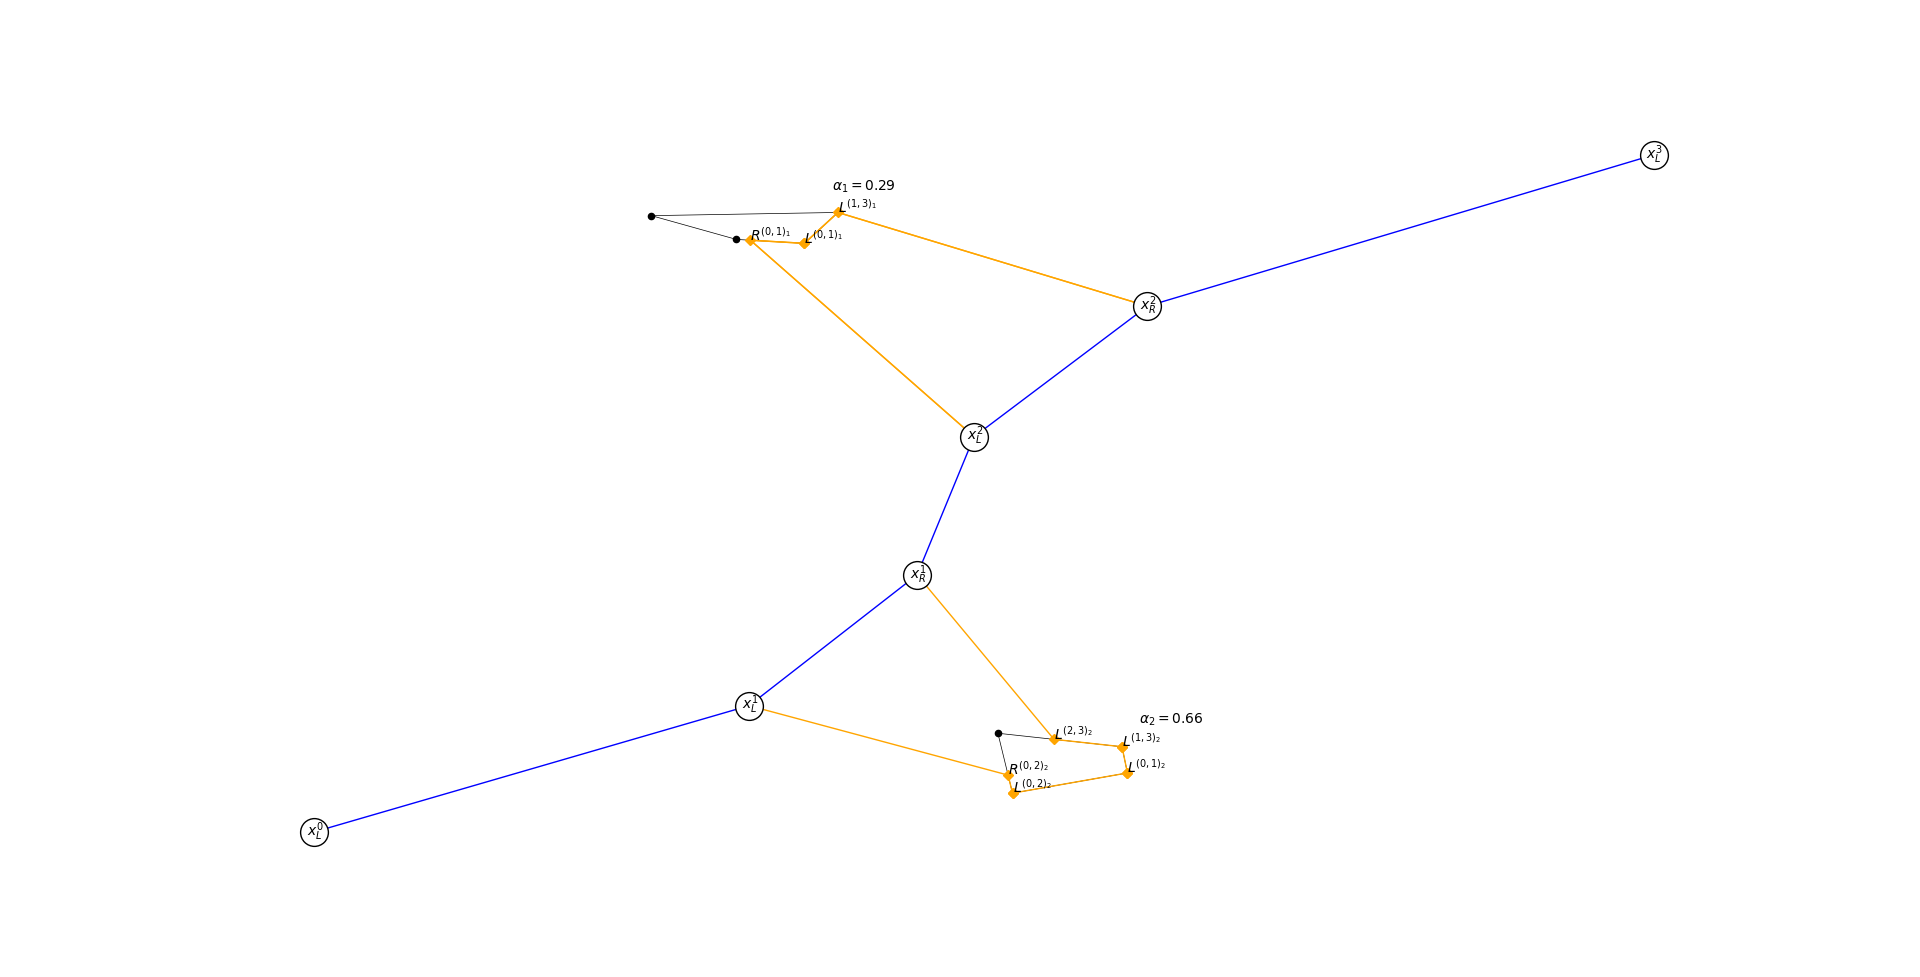
\includegraphics[height=9cm,width=\textwidth]{AMDRPG2.png}
\caption{Example illustrating the meaning of the launching  (L) and retrieving (R)  points. \label{fig:illustrative}}
\end{figure}

\JP{Figure \ref{fig:illustrative} shows an example of a configuration with two target graphs with four  nodes and four edges.%: one with six nodes and 7 edges and the other one with four nodes and edges%. 
The mothership begins at its starting point $x_L^0$. Then, it moves to $x_L^1$ where the drone is launched to visit the graph 2. There, the drone follows a route that ensures the coverage of $0.66 \%$ of the entire graph and returns to the point $x_R^2$ from where it is launched again to visit the second graph. Once, this graph is visited the drone returns to the mothership at the rendezvous point $x_R^2$ and so on ... }


\JP{In this formulation of \AMD the goal of is again to find a feasible solution that minimizes the total distance traveled  by the drone and  the mothership but without using stages. Instead the model ensures the Hamiltonian nature of the routes using the rationale of connectivity by the MTZ or SEC family of constraints. Therefore, modifying the previous formulation \sf{AMDRPG-ST}, replacing constraints based on stages, one obtains the following alternative valid formulation.}
\begin{mini*}|s|
 {}{\sum_{i_g} (u^{i_g}d_L^{i_g} + v^{i_g}d_R^{i_g}) + \sum_{i_g} d^{i_g} + \sum_{i_g,j_g}z^{i_gj_g}d^{i_gj_g} + \sum_g d_{LR}^g + \sum_{g,g'}d_{RL}^{gg'}w^{gg'}}{}{}\label{AMDRPG-MTZ}\tag{AMDRPG-MTZ}
 \addConstraint{\eqref{DEnt2}-\eqref{DInv2}}{}{}
 \addConstraint{\eqref{TOrig}-\eqref{TEnt}}{}{}
 \addConstraint{\eqref{MTZ1} - \eqref{MTZ2} \text{ or } \eqref{SEC} }{}{}
%\addConstraint{\eqref{MTZ3} - \eqref{MTZ6} \text{ or } \eqref{SEC} }{}{}   
 \addConstraint{\eqref{MTZ3} - \eqref{MTZ6}}{}{}   
 \addConstraint{\eqref{eq:alpha-E} \text{ or } \eqref{eq:alpha-G}}{}{}
 \addConstraint{\|x_L^g- R^{i_g}\|}{\leq d_L^{i_g},\quad}{\forall i_g}{}
 \addConstraint{\|R^{i_g}- L^{i_g}\|}{\leq d^{i_g},\quad}{\forall i_g}{}
 \addConstraint{\|R^{i_g}- L^{j_g}\|}{\leq d^{i_gj_g},\quad}{\forall i_g,j_g}{}
 \addConstraint{\|L^{i_g}- x_R^g\|}{\leq d_R^{i_g},\quad}{\forall i_g}{}
 \addConstraint{\|x_R^g- x_L^{g'}\|}{\leq d^{gg'}_{RL},\quad}{\forall g,g'}{}
 \addConstraint{\|x_L^g- x_R^g\|}{\leq d^g_{LR},\quad}{\forall g}{}
 \addConstraint{\left(\sum_{i_g} u^{i_g}d_L^{i_g} + \sum_{i_g, j_g}z^{i_gj_g}d^{i_gj_g} + \sum_{i_g} \mu^{i_g} d^{i_g} + \sum_{i_g}v^{i_g}d_R^{i_g}\right)/v_D}{\leq d_{RL}^{g}/v_M, \quad}{\forall g}{}\label{ACW}\tag{DCW}
 \addConstraint{x_L^0}{= orig}{}
 \addConstraint{x_R^0}{= orig}{}
 \addConstraint{x_L^{|\mathcal G|+1}}{= dest}{}
 \addConstraint{x_R^{|\mathcal G|+1}}{= dest.}{}
\end{mini*}


\JP{The formulation above \eqref{AMDRPG-MTZ} can be slightly modified replacing constraints $\eqref{MTZ3} - \eqref{MTZ6}$ by 
\begin{equation}\label{SEC-graph}
\sum_{g,g'\in \mathcal G} w^{gg'} \le |S|-1, \quad \forall S\subseteq \{1,\ldots, |\mathcal G|\}.
\end{equation}
This way we obtain another formulation for \AMD using SEC rather than MTZ constraints to represent the mothership tour. We will call this formulation (AMDRPG-SEC). Later, we will compare their performance in the computational results section.


\subsubsection{Comparing the formulations\label{ss:compare}}
A straightforward analysis of the two types of formulations, namely by stages and based on connectivity, shows that \ref{AMDRPG-MTZ} has much less variables and constraints than \ref{AMDRPG-ST}. Indeed, the latter requires definition of distance variables for each $i_g$ and $t$ which is a quadratic number rather than a linear one as used by the former. In addition, to enforce coordination \ref{AMDRPG-ST} needs constraints (DCW) for each $g\in \mathcal{G},\ t=1,\ldots,T$ whereas \ref{AMDRPG-MTZ} only uses (DCW) constraints for $g\in \mathcal{G}$. This is an important decrease in the dimension of the problems to be solved. This observation is confirmed in efficiency in problem solving in the section of computational experiments.} 


\subsection{Network Mothership-Drone Routing Problem on a Polygonal with Graphs (\PMD)}
The most significant difference between \AMD and  \PMD \ is that, in the latter, the mothership cannot move freely in $\mathbb R^2$ but it has to move on a network that models a road system where the mothership (truck) is restricted to move. \JP{An intermediate situation between moving freely and moving on a general road network is to assume that the mothership moves on a closed polygonal, namely a piecewise linear, chain. Modeling this situation is a transition step to achieve the more general case of the mothership moving on general networks. We will present the results for the \PMD \  following a scheme similar to that of \AMD. First, we present a model by stages and then another one based on connectivity constraints.}

Let $\mathcal P$ denote a polygonal chain parametrized by its breakpoints $A_1, \ldots, A_p$ ordered in the direction of travel. Observe that we are assuming that there exists a pre-specified orientation that determines the direction of the mothership's displacement. Let also $\gamma_L^{et}$ and $\gamma_R^{et}$ be the parameter values that define the points $x_L^t$ and $x_R^t$ on the edge $e$ on $\mathcal P$, respectively. \JP{Figure \ref{fig:ex1} illustrates the meaning of the parameters $\gamma_L^{et}$ and $\gamma_R^{et}$ on a polygonal chain with 4 pieces.} Then, the distance measured on the polygonal can be obtained by the following expressions:
\begin{equation}\tag{$d^{t\mathcal P}_{LR}$}\label{eq:dLRPt}
d_{LR}^{ee't} = \left\{\begin{matrix}
(\gamma_R^{et} - \gamma_L^{et})\mathcal L(e), & \text{if } e = e',\\ 
(1 - \gamma_L^{et})\mathcal L(e) + \sum_{e'' = e+1}^{e'-1}\mathcal L(e'') + \gamma_{R}^{e't}\mathcal L(e')), & \text{if } e < e'.
\end{matrix}\right.
\end{equation}

\begin{equation}\tag{$d^{t\mathcal P}_{RL}$}\label{eq:dRLPt}
d_{RL}^{ee't} = \left\{\begin{matrix}
(\gamma_{L}^{et+1}-\gamma_R^{et})\mathcal L(e), & \text{if } e = e',\\ 
(1 - \gamma_R^{et})\mathcal L(e) + \sum_{e'' = e+1}^{e'-1}\mathcal L(e'') + \gamma_{L}^{e't+1}\mathcal L(e')), & \text{if } e < e'.
\end{matrix}\right.
\end{equation}

This distance requires a binary variable $z_{LR}^{ee't}$ that determines whether $d_{LR}^{ee'}$ is defined by the first or the second expression in the formula:
$$z_{LR}^{ee't} = 1 \text{ if } \mu_{L}^{et} = 1 \text{ and }\mu_{R}^{e't} = 1,$$

\noindent where $\mu_{L}^{et}$ and $\mu_{R}^{et}$ are indicator variables that attain the value one if the launch point (resp. retrieve point) is placed in the segment $e$ of $\mathcal P$ at the stage $t$.

Similarly, we define $z_{RL}^{ee't}$:
$$z_{RL}^{ee't} = 1 \text{ if } \mu_{R}^{et} = 1 \text{ and }\mu_{L}^{e't+1} = 1.$$

In addition, we need to define continuous variables $\lambda_R^t$ and $\lambda_L^t$ that model the absolute position of the point $x_L^t$ in the polygonal to ensure that the movement of the mothership goes always in the allowed direction of travel and never comes back when it traverses the polygonal chain. 

\begin{figure}[h!]
\begin{center}
 \includegraphics[width=1\linewidth]{TDRPG.png}
\end{center}
\caption{An example of a parameterization of a mothership route that goes from $A_1$ to $x_L^t$ to launch the drone, then moves to $x_R^t$ on the edge $\overline{A_1A_2}$ to retrieve it, then it goes to $x_L^t$ on $\overline{A_2A_3}$ to launch it again, and travels until $x_R^t$ on $\overline{A_3A_4}$ to retrieve the drone and returns to the starting point at $A_1$.\label{fig:ex1}}
\end{figure}

With all this, we can model the movement of the mothership on the polygonal. For each stage $t$, we have

\begin{align}
    x_L^t & = \sum_{e=(i, i+1)\in\mathcal P} \mu_{L}^{et}\left[A^i + \gamma_L^{et}(A^{i+1} - A^i)\right]\label{param1}\\
    x_R^t & = \sum_{e=(i, i+1)\in\mathcal P} \mu_{R}^{et}\left[ A^i + \gamma_R^{et}(A^{i+1} - A^i)\right]\label{param2}\\
    z_{LR}^{ee't} & = \mu_{L}^{et}\mu_{R}^{e't}\label{pol:prodLR}\\
    z_{RL}^{ee't} & = \mu_{R}^{et}\mu_{L}^{e't+1}\label{pol:prodRL}\\
    \sum_{e} \mu_{L}^{et} & = 1  \label{muL} \\
    \sum_{e} \mu_{R}^{et} & = 1 \label{muR}\\
    d_{LR}^t & = \sum_{e, e'} z_{LR}^{ee't} d_{LR}^{ee'} \label{pol:dLRt},\\
    d_{RL}^t & = \sum_{e, e'} z_{RL}^{ee't} d_{RL}^{ee't} \label{pol:dRLt},\\
    \lambda_L^t - i & \geq \mu_{L}^{et} - (p-1)(1-\mu_{L}^{et}), \quad \forall e=(i, i+1)\in\mathcal P \label{lambdaLg}\\
    \lambda_L^t - i & \leq \mu_{L}^{et} - (p-1)(1-\mu_{L}^{et}), \quad \forall e=(i, i+1)\in\mathcal P \label{lambdaLl}\\
    \lambda_R^t - i & \geq \mu_{R}^{et} - (p-1)(1-\mu_{R}^{et}), \quad \forall e=(i, i+1)\in\mathcal P \label{lambdaRg}\\
    \lambda_R^t - i & \leq \mu_{R}^{et} + (p-1)(1-\mu_{R}^{et}), \quad \forall e=(i, i+1)\in\mathcal P \label{lambdaRl}\\
    \lambda_R^t & \geq \lambda_L^t \label{lambdaRL}\\
    \lambda_L^{t+1} & \geq \lambda_R^t \label{lambdaLR}
\end{align}

\noindent where $d_{LR}^{ee'}$ and $d_{RL}^{ee't}$ are defined in \eqref{eq:dLRPt} and \eqref{eq:dRLPt}. Constraints \eqref{param1} and \eqref{param2} parameterize the launch and retrieve points on the polygonal chain. Constraints \eqref{pol:prodLR} and \eqref{pol:prodRL} model the product of binary variables. Constraints \eqref{muL} and \eqref{muR} state that, in each stage, the launch and retrieve points can be only in one segment, not necessarily the same. Constraints \eqref{pol:dLRt} and \eqref{pol:dRLt} compute the total distance between the launch and the retrieve point in each stage. Inequalities \eqref{lambdaLg}-\eqref{lambdaRl} link $\mu_{L}^{et}$ and $\lambda_L^t$ (resp. $\mu_{R}^{et}$ and $\lambda_R^t$). Finally, constraints \eqref{lambdaRL} and \eqref{lambdaLR} ensure that the mothership moves in the right direction on the polygonal. Note that, in this case, it is not required to account for the distance $d_{RL}^t$ because by the assumptions on the model the mothership will traverse all the polygonal chain (since we have imposed that the route starts and ends at the same point).


The goal of the (\PMD) is, once again, to find a feasible solution that minimizes the total distance covered by the mothership and the drone. Thus, gathering all the above constraints one gets the following valid formulation.
\begin{mini*}|s|
 {}{\sum_{i_g, t} (u^{i_gt}d_L^{i_gt} + v^{i_gt}d_R^{i_gt}) + \sum_{i_g} d^{i_g} + \sum_{i_g,j_g}z^{i_gj_g}d^{i_gj_g} + \sum_t (d_{RL}^t + d_{LR}^t)}{}{}\tag{PMDRPG}
 \addConstraint{\eqref{st:DEnt}-\eqref{st:DInv}}{}{}
 \addConstraint{\eqref{param1}-\eqref{lambdaLR}}{}{}
 \addConstraint{\eqref{MTZ1} - \eqref{MTZ2} \text{ or } \eqref{SEC} }{}{}
 \addConstraint{\eqref{eq:alpha-E} \text{ or } \eqref{eq:alpha-G}}{}{}
 \addConstraint{\eqref{eq:dLRPt}, \eqref{eq:dRLPt}}{}{}
 \addConstraint{\|x_L^t- R^{i_g}\|}{\leq d_L^{i_gt},\quad}{\forall i_g,t}{}
 \addConstraint{\|R^{i_g}- L^{i_g}\|}{\leq d^{i_g},\quad}{\forall i_g,t}{}
 \addConstraint{\|R^{i_g}- L^{j_g}\|}{\leq d^{i_gj_g},\quad}{\forall i_g,j_g}{}
 \addConstraint{\|L^{i_g}- x_R^t\|}{\leq d_R^{i_gt},\quad}{\forall i_g,t}{}
 \addConstraint{\hspace*{-1.5cm} \left(\sum_{i_g} u^{i_gt}d_L^{i_gt} + \sum_{i_g, j_g}z^{i_gj_g}d^{i_gj_g} + \sum_{i_g} \mu^{i_g}d^{i_g} + \sum_{i_g} v^{i_gt}d_R^{i_gt}\right)/v_D}{\leq d_{RL}^t/v_M + M(1 - \sum_{i_g} u^{i_gt}), \,}{\forall g, t}{}\label{ACW}\tag{{\scriptsize DCW}}
 \addConstraint{x_L^0}{= orig}{}
 \addConstraint{x_R^0}{= orig}{}
 \addConstraint{x_L^{|\mathcal G|+1}}{= dest}{}
 \addConstraint{x_R^{|\mathcal G|+1}}{= dest.}{}
\end{mini*}
\subsubsection{Alternative formulation for \PMD \  based on MTZ-constraints}

\JP{Analogously to the case of \AMD one can also model \PMD \ without any explicit reference to stages. Here, we will follow a very similar approach to that in Section \ref{sec:AMDMTZ} to describe the formulation for \PMD \ based on MTZ-constraints.}

Let $\mathcal P$ denote, as before,  the polygonal chain parametrized by its endpoints $A_1, \ldots, A_p$ ordered in the direction of travel. In addition, let also $\gamma_{L}^{eg}$ and $\gamma_{R}^{eg}$ be the parameter values that define the points $x_L^g$ and $x_R^g$ on the line segment $\overline{A_iA_{i+1}}$ in $\mathcal P$, respectively. \JP{Then, the distance traveled on the polygonal can be obtained by one of  the following expressions. The first one refers to distances covered by the mothership between the launching and retrieving points of a drone operation, whereas models the distance traveled by the mothership between the launching and retrieving points of two consecutive graphs targeted in its route.}
\begin{equation}\tag{$d_{LR}^{g\mathcal P}$}\label{eq:dLRPg}
d_{LR}^{ee'g} = \left\{\begin{matrix}
|\gamma_{L}^{eg} - \gamma_{R}^{eg}|\mathcal L(e), & \text{if } e = e',\\ 
(1 - \gamma_{L}^{eg})\mathcal L(e) + \sum_{e'' =e+1}^{e'-1}\mathcal L(e'') + \gamma_{R}^{e'g}\mathcal L(e'), & \text{if } e < e', \\
\gamma_{L}^{eg}\mathcal L(e) + \sum_{e'' = e+1}^{e'-1}\mathcal L(e'') + (1-\gamma_{R}^{e'g})\mathcal L(e'), & \text{if } e > e'.
\end{matrix}\right.
\end{equation}

\begin{equation}\tag{$d_{RL}^{g\mathcal P}$}\label{eq:dRLPg}
d_{RL}^{ee'gg'} = \left\{\begin{matrix}
|\gamma_{L}^{eg} - \gamma_{R}^{eg'}|\mathcal L(e), & \text{if } e = e',\\ 
(1 - \gamma_{R}^{eg})\mathcal L(e) + \sum_{e'' = e+1}^{e'-1}\mathcal L(e'') + \gamma_{L}^{e'g'}\mathcal L(e'), & \text{if } e < e',\\
\gamma_{R}^{eg}\mathcal L(e) + \sum_{e'' = e+1}^{e'-1}\mathcal L(e'') + (1-\gamma_{L}^{e'g'})\mathcal L(e'), & \text{if } e > e'.
\end{matrix}\right.
\end{equation}

\JP{This distance requires binary variables $z_{LR}^{ee'g}$ and $z_{RL}^{ee'gg'}$ that determines which of the expressions in \eqref{eq:dLRPg} and  \eqref{eq:dRLPg} define $d_{LR}^{ee'g}$ and $d_{RL}^{ee'gg'}$,respectively.}
$$z_{LR}^{ee'g} = 1 \text{ iff } \mu_{L}^{eg} = 1 \text{ and }\mu_{R}^{e'g} = 1,\qquad
z_{RL}^{ee'gg'} = 1 \text{ iff } \mu_{L}^{eg} = 1 \text{ and }\mu_{R}^{e'g'} = 1,
$$
where $\mu_{L}^{eg}$ and $\mu_{R}^{eg}$ are indicator variables that attain the value one if the launch point (resp. retrieve point) associated to the graph $g$ is placed in the segment $\overline{A_iA_{i+1}}$ of the edge $e=(i, i+1) \in \mathcal P$ .

With all this, we can model the movement of the mothership inside the polygonal. 

\begin{align}
    x_L^g & = \sum_{e=(i, i+1)\in\mathcal P} \mu_{L}^{eg}\left[A^i + \gamma_L^{eg}(A^{i+1} - A^i)\right]\label{param1g}\\
    x_R^g & = \sum_{e=(i, i+1)\in\mathcal P} \mu_{R}^{eg}\left[ A^i + \gamma_R^{eg}(A^{i+1} - A^i)\right]\label{param2g}\\
    z_{LR}^{ee'g} & = \mu_{L}^{eg}\mu_{R}^{e'g}\label{prodLRg}\\
    z_{RL}^{ee'gg'} & = \mu_{R}^{eg}\mu_{L}^{e'g'}\label{prodRLg}\\
    \sum_{e} \mu_{L}^{eg} & = 1  \label{muLg} \\
    \sum_{e} \mu_{R}^{eg} & = 1 \label{muRg}\\
    d_{LR}^{g} & = \sum_{e, e'} z_{LR}^{ee'g} d_{LR}^{ee'g} \label{dLRg},\\
    d_{RL}^{gg'} & = \sum_{e, e'} z_{RL}^{ee'gg'} d_{RL}^{ee'gg'} \label{dRLgg},
\end{align}

\noindent where $d_{LR}^g$ and $d_{RL}^{gg'}$ are defined in \eqref{eq:dLRPg} and \eqref{eq:dRLPg}, respectively. Constraints \eqref{param1g} and \eqref{param2g} parameterize the launch and retrieve points on the polygonal chain. Constraints \eqref{prodLRg} and \eqref{prodRLg} model the product of binary variables. Constraints \eqref{muLg} and \eqref{muRg} state that, in each stage, the launch and retrieve points can be only in one segment, not necessarily the same. Constraints \eqref{dLRg} and \eqref{dRLgg} compute the total distance between the launch and the retrieve point for each pair of points. \JP{The reader may note that the above representation is similar to that given by \eqref{param1}-\eqref{pol:dRLt} with the exception that in \eqref{param1g}-\eqref{dRLgg} constraints are indexed in the set of graphs $g\in \mathcal{G}$ instead that on the stages. This fact allows a remarkable reduction on the number of distance variables and constraints as already discussed in Section \ref{ss:compare}.}

The goal of the (\PMD) is to find a feasible solution that minimizes the total distance covered by the drone and the mothership, i.e.,
\begin{mini*}|s|
 {}{\sum_{i_g} (u^{i_g}d_L^{i_g} + v^{i_g}d_R^{i_g}) + \sum_{i_g} d^{i_g} + \sum_{i_g,j_g}z^{i_gj_g}d^{i_gj_g} + \sum_g d_{LR}^g + \sum_{g,g'}d_{RL}^{gg'}w^{gg'}}{}{}\label{PMDRPG-MTZ}\tag{PMDRPG-MTZ}
 \addConstraint{\eqref{DEnt2}-\eqref{DInv2}}{}{}
 \addConstraint{\eqref{TOrig}-\eqref{TEnt}}{}{}
 \addConstraint{\eqref{MTZ1} - \eqref{MTZ2} \text{ or } \eqref{SEC} }{}{}
 \addConstraint{\eqref{MTZ3} - \eqref{MTZ6} \text{ or } \eqref{SEC} }{}{}   
 \addConstraint{\eqref{param1g}-\eqref{dRLgg}}{}{}
 \addConstraint{\eqref{eq:alpha-E} \text{ or } \eqref{eq:alpha-G}}{}{}
  \addConstraint{\eqref{eq:dLRPg}, \eqref{eq:dRLPg}}{}{}
 \addConstraint{\|x_L^g- R^{i_g}\|}{\leq d_L^{i_g},\quad}{\forall i_g}{}
 \addConstraint{\|R^{i_g}- L^{i_g}\|}{\leq d^{i_g},\quad}{\forall i_g}{}
 \addConstraint{\|R^{i_g}- L^{j_g}\|}{\leq d^{i_gj_g},\quad}{\forall i_g}{}
 \addConstraint{\|L^{i_g}- x_R^i\|}{\leq d_R^{i_g},\quad}{\forall i_g}{}
 \addConstraint{\left(\sum_{i_g} u^{i_g}d_L^{i_g} + \sum_{i_g, j_g}z^{i_gj_g}d^{i_gj_g} + \sum_{i_g} \mu^{i_g} d^{i_g} + \sum_{i_g}v^{i_g}d_R^{i_g}\right)/v_D}{\leq d_{RL}^{g}/v_M, \quad}{\forall g}{}\label{ACW}\tag{DCW}
 \addConstraint{x_L^0}{= orig}{}
 \addConstraint{x_R^0}{= orig}{}
 \addConstraint{x_L^{|\mathcal G|+1}}{= dest}{}
 \addConstraint{x_R^{|\mathcal G|+1}}{= dest.}{}
\end{mini*}

\JP{The reader may note that the above formulation actually encloses two different ones depending whether it includes constraints \eqref{MTZ1} - \eqref{MTZ2}  or  \eqref{SEC}. However, for the sake of presentation we have preferred to present them in this compact form to reduce the length of the paper.}

\subsection{Network Mothership-Drone Routing Problem with Graphs (\NMD)}
\JP{This new model is a refinement of the last one in that now the mothership has to move on a general undirected network rather than on a polygonal chain. 
Even though the previous one, namely \PMD, can be seen as a particular case of \NMD, for the sake of presentation, we have preferred to include it first to ease the understanding of the more advanced \NMD \ model.

As before, we start with an approach that models the problems by stages. Later, we shall extend the analysis using the rationale of connectivity, as already done in the the previous models \AMD \ and \PMD.}

Let $\mathcal N=(V, E)$ be the network that model the space of movement for the mothership. For each stage $t\in \{1,\ldots,|\mathcal G|\}$, assume that the mothership starts and ends in the edge $e=(i,j)$ and $e'=(i',j')$, respectively. Then, it follows a route from the launching to the retrieving point and vice versa, determined by a sequence of intermediate vertices, similar to the following one:

$$
e=(i, j) \ni x_L^t \rightarrow V_i \vee V_j \rightarrow \ldots \rightarrow V_k \rightarrow \ldots \rightarrow V_{i'} \rightarrow x_R^t \in (i',j')=e'.
$$
\JP{**** \@ Carlos: La notacion de $V_i$ y $i$ es un lio. Esto hay que aclararlo. *****}
Therefore, the distance traveled by the mothership, between two consecutive launching and retrieving points in two edges, not necessarily distinct,  of the graph can be represented as:
\begin{equation}\tag{$d^{t\mathcal N}_{LR}$}\label{eq:dLRNt}
d_{LR}^{ee't} = \left\{\begin{matrix}
|\gamma_{L}^{et} - \gamma_{R}^{et}|\mathcal L(e), & \text{if } e = e',\\ 
\left[b_{LR}^{it}\gamma_{L}^{et} + b_{LR}^{jt}(1 - \gamma_{L}^{et})\right]\mathcal L(e) + \displaystyle \sum_{e''\in \mathcal N}q_{LR}^{e''t}\mathcal L(e'') + \left[c_{LR}^{i't}\gamma_{R}^{e't} + c_{LR}^{j't}(1 - \gamma_{R}^{e't})\right]\mathcal{L}(e'), & \text{if } e \neq e',
\end{matrix}\right.
\end{equation}

\noindent 
where $b_{LR}^{it}$ (resp. $c_{LR}^{it}$) are binary variables that determine from which of the end-points of $e$ (respectively $e'$) one has to account for the distance and $q_{LR}^{et}$ is a binary variable that is one when the mothership fully traverses the edge $e$. \JP{Furthermore, we need to define another binary variable $z_{LR}^{ee't}$ that models the correct definition of the distance in \eqref{eq:dLRNt}. With the above definition one can account for  the movement of the mothership at each stage $t\in \{1, \ldots, |\mathcal G|\}$ from a launching to a retrieving  point:}

\begin{align}
    x_L^t & = \sum_{e=(i, j)\in E} \mu_{L}^{et}\left[V^i + \gamma_{L}^{et}(V^j - V^i)\right]\label{st:param1bis}\\
    x_R^t & = \sum_{e=(i, j)\in E} \mu_{R}^{et}\left[ V^i + \gamma_{R}^{et}(V^j - V^i)\right]\label{st:param2bis}\\
    z_{LR}^{ee't} & = \mu_{Le}^t\mu_{Re'}^t,\label{st:prodLRbis}\\
    b_{LR}^{it} & \leq \sum_{e\in\delta(i)}\mu_{L}^{et}, \label{st:bLt1}&\qquad\forall i\in V \\
    c_{LR}^{it} & \leq \sum_{e\in\delta(i)}\mu_{R}^{et}, \label{st:cLt1}&\qquad\forall i\in V\\
    b_{LR}^{it} + b_{LR}^{jt} & \geq \sum_{e'\neq e} z_{LR}^{ee't}, &\qquad \forall e=(i, j)\in E\label{st:bLt2}\\
    c_{LR}^{it} + c_{LR}^{jt} & \geq \sum_{e'\neq e} z_{LR}^{e'et}, &\qquad \forall e=(i, j)\in E\label{st:cLt2}\\
    b_{LR}^{it} + \sum_{\{j:(i, j)\in E\}} q_{LR}^{jit} & = \sum_{\{j:(i, j)\in E\}} q_{LR}^{ijt} +  c_{LR}^{it}, \label{st:flow}&\qquad \forall i \in V\\
    \sum_{e\in E} \mu_{L}^{et} & = 1,  \label{st:muLe} \\
    \sum_{e\in E} \mu_{R}^{et} & = 1, \label{st:muRe}\\
    d_{LR}^t & = \sum_{e, e'} z_{LR}^{ee't} d_{LR}^{ee't}, \label{st:dLRt}
\end{align}

Constraints \eqref{st:param1bis} and \eqref{st:param2bis} parameterize the launching and retrieving points in the network $\mathcal N$ at stage $t$. Constraints \eqref{st:prodLRbis} model the product of binary variables. Constraints \eqref{st:bLt1} and \eqref{st:cLt1} say that if the launching point (resp. retrieving point) is not in the edge $e$, the mothership cannot go (resp. exit) to the vertex that is incident to $e$. Constraints \eqref{st:bLt2} state that if the mothership leaves the edge $e$ to go to $e'$, it must exit from one of the incident vertices to $e$. In the same way, restrictions \eqref{st:cLt2} express that if the mothership leaves the edge $e'$ to go to $e$, it must enter to the edge $e$ from one of its incident vertices. Flow conservation constraints \eqref{st:flow} ensure that the number of incoming edges to each vertex $i$ is equal to the number of outgoing edges in the route followed by the mothership. Constraints \eqref{st:muLe} and \eqref{st:muRe} say that, in each stage, the selected points can be only in one edge. Finally, constraints \eqref{st:dLRt} defines the total distance between the launching and the retrieving points at  stage $t$.

\medskip

Similarly, the distance covered by the mothership along the path on the network from the retrieving point $x_R^t$ to the next launching point $x_L^{t+1}$ can be modeled using the following definition of distance:

\begin{equation}\tag{$d^{t\mathcal N}_{RL}$}\label{eq:dRLNt}
d_{RL}^{ee't} = \left\{\begin{matrix}
|\gamma_{R}^{et} - \gamma_{L}^{et+1}|\mathcal L(e), & \text{if } e = e',\\ 
\left[b_{RL}^{it}\gamma_{R}^{et} + b_{RL}^{jt}(1 - \gamma_{R}^{et})\right]\mathcal L(e) + \displaystyle \sum_{e''\in \mathcal N}q_{RL}^{e''t}\mathcal L(e'') + \left[c_{RL}^{i't}\gamma_{L}^{e't+1} + c_{RL}^{j't}(1 - \gamma_{L}^{e't+1})\right]\mathcal{L}(e'), & \text{if } e \neq e'.
\end{matrix}\right.
\end{equation}

In this case, the binary variable $z_{ee'}^{RLt}$ links the retrieve point at $t$ with the launch point at $t+1$. Then, we can use a set of constraints similar to those used above and the distance from $x_R^t$ to $x_L^{t+1}$ is:

\begin{align}
    z_{RL}^{ee't} & = \mu_{R}^{et}\mu_{L}^{e't+1},\label{st1:prodRL}\\
    b_{RL}^{it} & \leq \sum_{e\in\delta(i)}\mu_{R}^{et}, \label{st1:bRt1}&\qquad \forall i\in V \\
    c_{RL}^{it} & \leq \sum_{e\in\delta(i)}\mu_{L}^{et}, \label{st1:cRt1}&\qquad \forall e\in\delta(i),\,\forall i\in V\\
    b_{RL}^{it} + b_{RL}^{jt} & \geq \sum_{e'\neq e} z_{RL}^{ee't}, &\qquad \forall e=(i, j)\in E\label{st1:bRt2}\\
    c_{RL}^{it} + c_{RL}^{jt} & \geq \sum_{e'\neq e} z_{RL}^{e'et}, &\qquad \forall e=(i, j)\in E\label{st1:cRt2}\\
    b_{RL}^{it} + \sum_{\{j:(i, j)\in E\}} q_{RL}^{jit} & = \sum_{\{j:(i, j)\in E\}} q_{RL}^{ijt} +  c_{RL}^{it}, \label{st1:flow}&\qquad \forall i \in V\\
    \sum_{e\in E} \mu_{L}^{et} & = 1,  \label{st1:muLe} \\
    \sum_{e\in E} \mu_{R}^{et} & = 1, \label{st1:muRe}\\
    d_{RL}^t & = \sum_{e, e'} z_{RL}^{ee't} d_{RL}^{ee't}. \label{st1:dRLtN}
\end{align}

\JP{Constraints \eqref{st1:prodRL} model the product of binary variables. Constraints \eqref{st1:bRt1} and \eqref{st1:cRt1} say that if the retrieving point (resp. launching point) is not in the edge $e$, the mothership cannot go (resp. exit) to the end vertices of the edge $e$. Constraints \eqref{st1:bRt2} state that if the mothership leaves the edge $e$ to go to $e'$, it must exit via one of the end vertices of $e$. In the same way, restrictions \eqref{st1:cRt2} state that if the mothership leaves the edge $e'$ to go to $e$, it necessarily must enter to $e$ from one incident vertex of $e$. Flow conservation constraints \eqref{st1:flow} ensure that in the route followed by the mothership the number of used incoming edges to each vertex $i$ is equal to the number of used outgoing edges. Constraints \eqref{st1:muLe} and \eqref{st1:muRe} say that, in each stage, the selected points can be only in one edge. Constraints \eqref{st1:dRLtN} state the total distance between the retrieving and the launching points at stage $t$.}


Hence, once the distances inside the graph are set with the above two families of constraints, we can state the mathematical programming formulation of the problem as:

\begin{mini*}|s|
 {}{\sum_{i_g, t} (u^{i_gt}d_L^{i_gt} + v^{i_gt}d_R^{i_gt}) + \sum_{i_g} d^{i_g} + \sum_{i_g,j_g}z^{i_gj_g}d^{i_gj_g} + \sum_t (d_{RL}^t + d_{LR}^t)}{}{}\tag{TDRPG}
 \addConstraint{\eqref{st:DEnt}-\eqref{st:DInv}}{}{}
 \addConstraint{\eqref{st:param1bis}-\eqref{st1:dRLtN}}{}{}
 \addConstraint{\eqref{eq:dLRNt}, \eqref{eq:dRLNt}}{}{}
 \addConstraint{\eqref{MTZ1} - \eqref{MTZ2} \text{ or } \eqref{SEC} }{}{}
 \addConstraint{\eqref{eq:alpha-E} \text{ or } \eqref{eq:alpha-G}}{}{}
 \addConstraint{\|x_L^t- R^{i_g}\|}{\leq d_L^{i_gt},\quad}{\forall i_g,t}{}
 \addConstraint{\|R^{i_g}- L^{i_g}\|}{\leq d_g^{i_g},\quad}{\forall i_g,t}{}
 \addConstraint{\|R^{i_g}- L^{j_g}\|}{\leq d^{i_gj_g},\quad}{\forall i_g,j}{}
 \addConstraint{\|L^{i_g}- x_R^i\|}{\leq d_R^{i_gt},\quad}{\forall i_g,t}{}
 \addConstraint{\hspace*{-2cm}\left(\sum_{i_g} u^{i_gt}d_L^{i_gt} + \sum_{i, j}z^{i_gj_g}d^{i_gj_g} + \sum_{i_g} \mu^{i_gt}d^{i_g} + \sum_{i_g} v^{i_gt}d_R^{i_gt}\right)/v_D}{\leq d_{RL}^t/v_M + M(1 - \sum_{i_g} u^{i_gt}),\ }{\forall g, t}{}\label{ACW}\tag{DCW}
 \addConstraint{x_L^0}{= orig}{}
 \addConstraint{x_R^0}{= orig}{}
 \addConstraint{x_L^{|\mathcal G|+1}}{= dest}{}
 \addConstraint{x_R^{|\mathcal G|+1}}{= dest.}{}
\end{mini*}

\JP{A brief decription of this formulation must be included ...}

\subsubsection{MTZ formulation for the Network Mothership-Drone Routing Problem with Graphs}

\JP{Something missing to connect it to the previous section ... JUSTO: Por aqui 20/11/2020}

Therefore, the distance between launching and retrieving points in two edges, not necessarily distinct,  of the graph can be represented as:
\begin{equation}\tag{$d^{g\mathcal N}_{LR}$}\label{eq:dLRg}
d_{LR}^{ee'g} = \left\{\begin{matrix}
|\gamma_{L}^{eg} - \gamma_{R}^{eg}|\mathcal L(e), & \text{if } e = e',\\ 
\left[b_{LR}^{ig}\gamma_{L}^{eg} + b_{LR}^{jg}(1 - \gamma_{L}^{eg})\right]\mathcal L(e) + \displaystyle \sum_{e''\in \mathcal N}q_{LR}^{e''g}\mathcal L(e'') + \left[c_{LR}^{i'g}\gamma_{R}^{e'g} + c_{LR}^{j'g}(1 - \gamma_{R}^{e'g})\right]\mathcal{L}(e'), & \text{if } e \neq e',
\end{matrix}\right.
\end{equation}

\noindent 
where $b_{LR}^{ig}$ (resp. $c_{LR}^{ig}$) are binary variables that determine from which of the end-points of $e$ (respectively $e'$) one has to account for the distance and $q_{LR}^{eg}$ is a binary variable that is one when the mothership fully traverses the edge $e$. Furthermore, we need to define binary variables $z_{LR}^{ee'g}$ that model the choice of the model for right definition (first or second formulas in \eqref{eq:dLRg}) of the distance in \eqref{eq:dLRg}. All the above give the necessary elements to account for the movement of the mothership in each graph $g\in \{1, \ldots, |\mathcal G|\}$:

\begin{align}
    x_L^g & = \sum_{e=(i, j)\in E} \mu_{L}^{eg}\left[V^i + \gamma_{L}^{eg}(V^j - V^i)\right]\label{g:param1bisg}\\
    x_R^g & = \sum_{e=(i, j)\in E} \mu_{R}^{eg}\left[ V^i + \gamma_{R}^{eg}(V^j - V^i)\right]\label{g:param2bisg}\\
    z_{LR}^{ee'g} & = \mu_{L}^{eg}\mu_{R}^{e'g},\label{g:prodLR}\\
    b_{LR}^{ig} & \leq \sum_{e\in\delta(i)} \mu_{L}^{eg}, \label{g:bLt1}&\qquad \forall i\in V \\
    c_{LR}^{ig} & \leq \sum_{e\in\delta(i)} \mu_{R}^{eg}, \label{g:cLt1}&\qquad \forall i\in V\\
    b_{LR}^{ig} + b_{LR}^{jg} & \geq \sum_{e'\neq e} z_{LR}^{ee'g}, &\qquad \forall e=(i, j)\in E\label{g:bLt2}\\
    c_{LR}^{ig} + c_{LR}^{jg} & \geq \sum_{e'\neq e} z_{LR}^{e'eg}, &\qquad \forall e=(i, j)\in E\label{g:cLt2}\\
    b_{LR}^{ig} + \sum_{\{j:(i, j)\in E\}} q_{LR}^{jig} & = \sum_{\{j:(i, j)\in E\}} q_{LR}^{ijg} +  c_{LR}^{ig}, \label{g:flow}&\qquad \forall i \in V\\
    \sum_{e\in E} \mu_{L}^{eg} & = 1,  \label{g:muLe} \\
    \sum_{e\in E} \mu_{R}^{eg} & = 1, \label{g:muRe}\\
    d_{LR}^g & = \sum_{e, e'} z_{LR}^{ee'g} d_{LR}^{ee'g}, \label{g:dLRgN}
\end{align}

\JP{Constraints \eqref{g:param1bisg} and \eqref{g:param2bisg} parameterize the launch and retrieve points in the network $\mathcal N$ induced by the visit to the graph  $g\in \mathcal{G}$. Constraints \eqref{g:prodLR} model the product of binary variables. Constraints \eqref{g:bLt1} and \eqref{g:cLt1} say that if the launch point (resp. retrieve point) is not in the edge $e$, the drone cannot go (resp. exit) to the vertices of the edge $e$. Constraints \eqref{g:bLt2} state that if the drone leaves the edge $e$ to go to $e'$, it must exit from one of the incident vertices to $e$. In the same way, restrictions \eqref{g:cLt2} express that if the drone leaves the edge $e'$ to go to $e$, it necessarily must enter to $e$ from one incident vertex of $e$. Flow conservation constraints \eqref{g:flow} ensure that the number of incoming edges to each vertex $i$ is equal to the number of outgoing edges. Constraints \eqref{g:muLe} and \eqref{g:muRe} say that, in visit to the graph  $g\in \mathcal{G}$, launching and retrieving points can be only in one edge. Constraints \eqref{g:dLRgN} returns the total distance traveled by the drone on the graph  $g\in \mathcal{G}$.}

\medskip

Similarly, the distance covered by the mothership along the path on the network from the retrieving point $x_R^g$ to the next launching point $x_L^{g'}$ can be modeled using the following definition of distance:

\begin{equation}\tag{$d^{g\mathcal N}_{RL}$}\label{eq:dRLg}
d_{RL}^{ee'gg'} = \left\{\begin{matrix}
|\gamma_{R}^{eg} - \gamma_{L}^{eg'}|\mathcal L(e), & \text{if } e = e',\\ 
\left[b_{RL}^{ig}\gamma_{R}^{eg} + b_{RL}^{jg}(1 - \gamma_{R}^{eg})\right]\mathcal L(e) + \displaystyle \sum_{e''\in \mathcal N}q_{RL}^{e''gg'}\mathcal L(e'') + \left[c_{RL}^{i'g'}\gamma_{L}^{e'g'} + c_{RL}^{j'g'}(1 - \gamma_{L}^{e'g'})\right]\mathcal L(e'), & \text{if } e \neq e'.
\end{matrix}\right.
\end{equation}

In this case, the binary variable $z_{RL}^{ee'gg'}$ links the retrieve point at $g$ with the launch point at $g'$. Then, we can use a set of constraints similar to those used above and the distance from $x_R^g$ to $x_L^{g'}$ is:

\begin{align}
    z_{RL}^{ee'gg'} & = \mu_{R}^{eg}\mu_L^{e'g'},\label{prodRLggN}\\
    b_{RL}^{ig} & \leq \mu_{R}^{eg}, \label{bRt1}&\qquad \forall e\in\delta(i),\,\forall i\in V \\
    c_{RL}^{ig} & \leq \mu_{L}^{eg}, \label{cRt1}&\qquad \forall e\in\delta(i),\,\forall i\in V\\
    b_{RL}^{ig} + b_{RL}^{jg} & \geq \sum_{e'\neq e} z_{RL}^{ee'gg'}, &\qquad \forall e=(i, j)\in E\label{bRt2}\\
    c_{RL}^{ig'} + c_{RL}^{jg'} & \geq \sum_{e'\neq e} z_{RL}^{e'eg'g}, &\qquad \forall e=(i, j)\in E\label{cRt2}\\
    b_{RL}^{ig} + \sum_{\{j:(i, j)\in E} q_{RL}^{jigg'} & = \sum_{\{j:(i, j)\in E\}} q_{RL}^{ijgg'} +  c_{RL}^{ig}, \label{flow}&\qquad \forall i \in V\\
    \sum_{e\in E} \mu_{L}^{eg} & = 1,  \label{muLe} \\
    \sum_{e\in E} \mu_{R}^{eg} & = 1, \label{muRe}\\
    d^{RLgg'} & = \sum_{e, e'} z_{RL}^{ee'gg'} d_{RL}^{ee'gg'}. \label{dRLt}
\end{align}

Hence, once the distances inside the graph are set with the above two families of constraints, we can state the mathematical programming formulation of the problem as:

\begin{mini*}|s|
 {}{\sum_{i, g, t} (u^{i_gt}d_L^{i_gt} + v^{i_gt}d_R^{i_gt}) + \sum_{i_g} d^{i_g} + \sum_{i,j,g}z^{i_gj_g}d^{i_gj_g}}{}{}\tag{TDRPG}
 \addConstraint{\eqref{st:DEnt}-\eqref{st:DInv}}{}{}
 \addConstraint{\eqref{g:param1bisg}-\eqref{dRLt}}{}{}
 \addConstraint{\eqref{eq:dLRg}, \eqref{eq:dRLg}}{}{}
 \addConstraint{\eqref{MTZ1} - \eqref{MTZ2} \text{ or } \eqref{SEC} }{}{}
 \addConstraint{\eqref{eq:alpha-E} \text{ or } \eqref{eq:alpha-G}}{}{}
 \addConstraint{\|x_L^t- R^{i_g}\|}{\leq d_L^{i_gt},\quad}{\forall i_g,t}{}
 \addConstraint{\|R^{i_g}- L^{i_g}\|}{\leq d_g^{i_g},\quad}{\forall i_g,t}{}
 \addConstraint{\|R^{i_g}- L^{j_g}\|}{\leq d^{i_gj_g},\quad}{\forall i_g,j}{}
 \addConstraint{\|L^{i_g}- x_R^i\|}{\leq d_R^{i_gt},\quad}{\forall i_g,t}{}
 \addConstraint{\left(\sum_{i_g} u^{i_g}d_L^{i_g} + \sum_{i, j}z^{i_gj_g}d^{i_gj_g} + \sum_{i_g} \mu^{i_g}d^{i_g} + \sum_{i_g} v^{i_g}d_R^{i_g}\right)/v_D}{\leq d_g^{RL}/v_M, \quad}{\forall g}{}\label{ACW}\tag{DCW}
 \addConstraint{x_L^0}{= orig}{}
 \addConstraint{x_R^0}{= orig}{}
 \addConstraint{x_L^{|\mathcal G|+1}}{= dest}{}
 \addConstraint{x_R^{|\mathcal G|+1}}{= dest.}{}
\end{mini*}
% $$
% e=(i, j) \ni x_R^t \rightarrow V_i \vee V_j \rightarrow \ldots \rightarrow V_k \rightarrow \ldots \rightarrow V_{i'} \rightarrow x_L^{t+1} \in (i',j')=e'
% $$

% The design of these paths obeys to define binary variables that decide which vertices are selected in each stage $t$: